\chapter{Algoritmi e loro complessità: i numeri di Fibonacci}

{~{[}DFI{]} cap. 1}

\begin{equation}
f(n) = 
\begin{cases}
1 & \mbox{se } n=1,n=2 \\ 
(n-1)+f(n-2) & \mbox{se } n\geq3 
\end{cases}
\end{equation}

\section{Formula di Binet}

\begin{equation}
\forall n \in N, F_n = \frac{1}{\sqrt{5}}(\Phi^n-\overline{\Phi}^n)
\end{equation}

Dove con $\Phi$ si indica la sezione aurea $\frac{1+\sqrt{5}}{2} \simeq -0,618$ e con $\overline{\Phi}$ si indica $\frac{1-\sqrt{5}}{2} \simeq -0,618$

\subsubsection{Dimostrazione}

{Dimostriamo per Induzione la formula di Binet:}

{Base:}

{$n = 1 \rightarrow F_n = \frac{1}{\sqrt{5}}(\Phi^1-\overline{\Phi}^1)$

{Sostistuisco con le definizioni di $\Phi$ e semplifico}

{$F_n = 1 = F_1$}

{$n = 2 \rightarrow F_n =\frac{1}{\sqrt{5}}(\Phi^2-\overline{\Phi}^2)$

{Sostistuisco con le definizioni di $\Phi$ e semplifico}

{$F_n = 1 = F_2$}

{Passo induttivo $n \geq 3$ :}

$F_n = F_{n-1} + F_{n-2}$

$F_{n-1}=\frac{1}{\sqrt{5}}(\Phi^{n-1}-\overline{\Phi}^{n-1})$ e 
$F_{n-2}=\frac{1}{\sqrt{5}}(\Phi^{n-2}-\overline{\Phi}^{n-2})$

{assomiglia alla forma $F_n=\frac{1}{\sqrt{5}}(\Phi^n-\overline{\Phi}^n)$}

{ci chiediamo se $\Phi^n=\Phi^{n-1}+\Phi^{n-2}$ e se $\overline{\Phi}^n=\overline{\Phi}^{n-1}+\overline{\Phi}^{n-2}$

{divido da entrambe le parti per $\Phi^{n-2}$ e $\overline{\Phi}^{n-2}$}

\paragraph{Definizione 1}

{Utilizzeremo la notazione $T_n$ per indicare la velocità/complessità di una particolare funzione (numero di righe di codice eseguite) }

\lstinputlisting{code/fib1.txt}

$T(Fib1)_n = 1\,\forall n$

{Problema: con l'aumentare di $n$, la funzione $Fib1(n)$ diventa sempre più imprecisa}

$Fib1_3=1,9999.. \simeq 2$ \\
$Fib1_{16}=986,699.. \simeq 987$ \\
$Fib1_{18}=2583,1.. \simeq 2584$

\paragraph{Definizione 2}

\lstinputlisting{code/fib2.txt}

\begin{equation}
T(Fib2)_n = 
\begin{cases}
1 & \mbox{se } n=1,n=2 \\ 
2 + T_{n-1} + T_{n-2} & \mbox{se } \forall n \geq 3 
\end{cases}
\end{equation}

{$T(Fib2)_n$ è una formula ricorsiva o ricorrenza}


\begin{tabular}{|c|c|}
\hline 
$n$ & $T_n$ \\ 
\hline 
1 & 1 \\ 
\hline 
2 & 1 \\ 
\hline 
3 & 2+1+1 = 4 \\ 
\hline 
4 & 2+4+1=7 \\ 
\hline 
5 & 2 + 7 + 4 = 13 \\ 
\hline 
\end{tabular} 

{Risolviamo la ricorrenza per determinare la complessità / bontà della funzione esaminata.}

\begin{itemize}
\tightlist
\item
  {andamento esponenziale rispetto ad $n$: funzione NON efficiente}
\item
  {andamento logaritmico / proporzionale rispetto ad $n$: funzione
  efficiente}
\end{itemize}

\begin{center}\rule{0.5\linewidth}{\linethickness}\end{center}

\subsubsection{Strumento 1 - Albero di ricorsione}

{Notiamo che $T(Fib2)_5=(1*5)+(2*4)=13$, dove $(1 * 5)$ è la complessità delle foglie (5 foglie con peso 1) e $(2 * 4)$ è la complessità dei nodi interni (4 nodi con peso 2)}

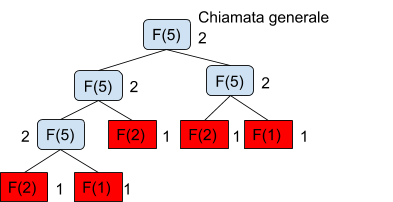
\includegraphics{images/image523.png}



\paragraph{Proprietà 1}

{Se $T_n$ rappresenta l'albero di ricorsione relativo a $Fib2_n$, allora il numero di foglie di $T_n$ è uguale a $F_n$(con $F_n$ indichiamo l'n-esimo numero della successione di Fibonacci)}

{Dimostrazione per induzione}

{Base:}

{se $n = 1$, il numero di foglie di $T_2$, $F_1=1$}

{se $n = 2$, il numero di foglie di $T_2$, $F_2=1$}

{Passo induttivo:}

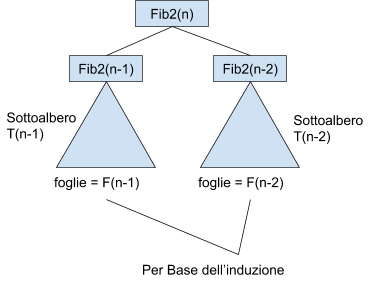
\includegraphics{images/image528.png}

\paragraph{Proprietà 2}

{Sia $T$ un albero binario in cui ogni nodo interno ha esattamente 2 figli}

{Allora $i_T=f_T-1$, dove con $i_T$ indichiamo il numero di nodi interni dell'albero $T$ e con $f_T$ indichiamo il numero di foglie dell'albero $T$}

\paragraph{Dimostrazione per induzione}

{Dimostrazione su $n$, dove $n$ è il numero di nodi di $T$}

{Base $n=1$ : OVVIO}

{Passo induttivo: $n \geq 2$}

{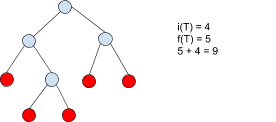
\includegraphics{images/image525.png}}

{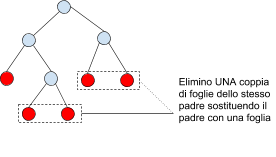
\includegraphics{images/image536.png}}

{L'albero risultante lo chiamiamo $\overline{T}$:}

{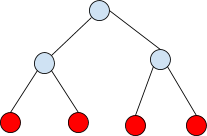
\includegraphics{images/image522.png}}

{Notiamo che }

$t_{\overline{T}} = f_{\overline{T}}-1${*}

$f_{\overline{T}} = f_{T}-1${**}

$i_{\overline{T}} = i_{T}-1$

{→ (inverto) $i_T=i_{\overline{T}}+1$}

{→ (sostituisco*) $i_T=f_{\overline{T}}+1-1$}

{→ (semplifico) $i_T=f_{\overline{T}}$}

{→ (sostituisco**) $i_T=f_T-1$}

{Studio complessità di $Fib2_n$ con l'utilizzo del metodo dell'albero di ricorsione}

$i_{T_n}=F_n-1$

$f_{T_n}=F_n$

$T_n = 2 * i_{T_n}+1*f_{T_n}$

{→ $2 * F_{n-1} + F_n$}

{→ $3 * F_n - 2$}

\paragraph{Proprietà 3}

\begin{equation}
\forall n \geq 6 \rightarrow F_n \geq 2^{\frac{n}{2}}
\end{equation}

{Dimostrazione per induzione}

{Base $n=6$ :}

$F_6=8$	\\
$2^{\frac{6}{3}}=2^3=8$

{Passo induttivo $n \geq 7$ :}

$F(n) \geq 2^{\frac{n-1}{2}} + 2^{\frac{n-2}{2}}$

$F(n) \geq 2^{\frac{n}{2}} * 2^{-\frac{1}{2}} + 2^{\frac{n}{2}} * 2^{-1} $

$F(n) \geq 2^{\frac{n}{2}} * ( 2^{-\frac{1}{2}} + 2^{-1} )$

{$2^{-\frac{1}{2}}+2^{-1}$ è sempre maggiore o uguale ad 1}

{$Fib2(n)$ risulta essere troppo poco efficiente}

$T(8)=61$

$T(45) = 3,404,709,508$

{Definiamo allora $Fib3(n)$ utilizzando l'iterazione al posto della ricorsione}

\lstinputlisting{code/fib3.txt}

$T(Fib3_n)=3+(n-2)+(n-1)=2n$

{Ci chiediamo se fib3 sia efficiente dal punto di vista della
memoria\ldots{}}
